\documentclass[11pt, a4paper]{article}
\usepackage[utf8]{inputenc}
\usepackage[spanish]{babel}
\usepackage{graphicx}
\usepackage{fancyhdr}
\usepackage{geometry}
\usepackage{amsmath, amssymb, amsfonts}
\usepackage{booktabs}
\usepackage{multirow}
\usepackage{enumitem}
\usepackage{xcolor}
\usepackage{hyperref}
\usepackage{natbib}
\usepackage{url}
\usepackage{tikz}
\usepackage{float}
\usepackage{microtype}

% Configuración de geometría de página
\geometry{margin=2.5cm, headheight=15pt}

% Configuración de colores
\definecolor{maincolor}{RGB}{0, 83, 134}
\definecolor{secondcolor}{RGB}{0, 124, 180}

% Configuración de hipervínculos
\hypersetup{
    colorlinks=true,
    linkcolor=maincolor,
    filecolor=maincolor,
    urlcolor=maincolor,
    citecolor=maincolor,
    pdftitle={Logística de Mercados y Redimensión en Rutas de Puno},
    pdfauthor={Universidad Nacional del Altiplano},
    pdfsubject={Métodos de Optimización},
    pdfkeywords={Programación Lineal Mixta, Logística, Optimización, Distribución de Gas}
}

% Estilo de página
\pagestyle{fancy}
\fancyhf{} % Limpia los encabezados y pies de página

% Encabezado
\fancyhead[L]{
\includegraphics[height=1cm]{LOGO.png}}
\fancyhead[C]{%
\begin{tabular}{c}
\textbf{\color{maincolor}\uppercase{Universidad Nacional del Altiplano}} \\ 
{\small FACULTAD DE INGENIERÍA ESTADÍSTICA E INFORMÁTICA}
\end{tabular}}
\fancyhead[R]{
\includegraphics[height=1cm]{logoinfo.png}}

% Pie de página
\fancyfoot[L]{\small \textit{MÉTODOS DE OPTIMIZACIÓN}} % texto a la izquierda
\fancyfoot[C]{\small \thepage} % Número de página centrado
\fancyfoot[R]{\small \textit{\today}} % fecha a la derecha

% Redefinición de secciones para mejor estética
\usepackage{titlesec}
\titleformat{\section}
  {\normalfont\Large\bfseries\color{maincolor}}{\thesection}{1em}{}
\titleformat{\subsection}
  {\normalfont\large\bfseries\color{secondcolor}}{\thesubsection}{1em}{}

\begin{document}

\begin{titlepage}
    \centering
    \vspace*{1cm}
    {
\includegraphics[width=0.3\textwidth]{LOGO.png}\par}
    \vspace{1.5cm}
    {\LARGE\bfseries\color{maincolor} UNIVERSIDAD NACIONAL DEL ALTIPLANO\par}
    \vspace{0.5cm}
    {\large FACULTAD DE INGENIERÍA ESTADÍSTICA E INFORMÁTICA\par}
    \vspace{1.5cm}
    {\Huge\bfseries\color{maincolor} SOLUCIÓN A LA LOGÍSTICA DE MERCADOS Y REDIMENSIÓN EN LAS RUTAS DE PUNO-PERÚ APLICANDO LA PROGRAMACIÓN LINEAL MIXTA\par}
    \vspace{1.5cm}
    {\Large\itshape Trabajo de Investigación\par}
    \vspace{1.0cm}
    {\large\bfseries Curso: \par}
    {\large MÉTODOS DE OPTIMIZACIÓN\par}
    {\large\bfseries Integrantes: \par}
    {\large Jimena Yessica Paricela Yana\par}
    {\large Etzel Yuliza Peralta Lopez \par}
    {\large Belinda Apaza Quispe\par}
    {\large Beatriz Umiña Machaca \par}
    \vfill
    {\large \today\par}
\end{titlepage}

\thispagestyle{fancy} % Usa el estilo en la página actual

\begin{abstract}
\noindent Los problemas de asignación de recursos escasos a tareas competitivas pueden resolverse eficientemente mediante procedimientos de programación lineal mixta. Estos procedimientos son apropiados siempre que las variables del problema estén relacionadas linealmente entre sí. Sus aplicaciones han sido extensas en la industria y algunas veces han proporcionado ahorros notables \citep{Hillier2010}. Aunque la programación lineal no es la única forma de optimizar las utilidades para un sistema dado, muchas de las relaciones fundamentales entre variables incitan a su utilización, especialmente en problemas de distribución y logística como el que se aborda en este trabajo \citep{Taha2017}.
\end{abstract}

\tableofcontents
\newpage

\section{Introducción}
En la gestión logística de la región de Puno, uno de los mayores retos es la distribución eficiente, efectiva y sostenible de recursos —como materiales, vehículos, personal e infraestructura— para atender toda la demanda regional \citep{Ballou2004}. La correcta distribución de los recursos es esencial para mejorar la cobertura de servicios, reducir costos y minimizar el impacto ambiental, en línea con los principios que plantea \citet{Nahmias2014} en el capítulo 5 del libro "Sistemas de Producción: Planeación, Análisis y Control".

Este capítulo aporta una fundamentación teórica que permite comprender la importancia de planificar, gestionar y optimizar la distribución de recursos en los procesos productivos y logísticos, un aspecto clave en el contexto regional de Puno. La aplicación de técnicas de investigación operativa, particularmente la programación lineal mixta, ofrece una oportunidad para mejorar significativamente la eficiencia de estas operaciones \citep{Winston2004}.

La distribución de gas licuado de petróleo (GLP) en Puno enfrenta desafíos logísticos significativos debido a la geografía compleja, altitud y clima variable de esta región altiplánica peruana. Con más del 70 porciento de hogares dependientes del GLP envasado según el MINEM (2023), este servicio resulta esencial pero complicado de gestionar eficientemente.

Las empresas distribuidoras locales suelen emplear métodos tradicionales sin optimización matemática, provocando problemas como demanda insatisfecha, uso ineficiente de vehículos y rutas subóptimas. Esta situación demanda la implementación de técnicas avanzadas de investigación operativa.

El presente estudio plantea un modelo de programación lineal mixta (MILP) basado en el Problema Integrado de Ruteo y Gestión de Inventario con Múltiples Vehículos (MVIRP). Su objetivo es optimizar la distribución de GLP en Puno, reduciendo costos operativos e incorporando criterios sostenibles como la minimización de emisiones y riesgos. Utilizando datos basados en parámetros reales, este enfoque busca mejorar la eficiencia distributiva y establecer un precedente para futuras aplicaciones logísticas en zonas geográficamente desafiantes.

\section{Propósito}
El propósito de esta investigación es desarrollar un modelo de programación lineal mixta (MILP) para optimizar las rutas de distribución de gas en la región de Puno, con el objetivo de:

\begin{itemize}[leftmargin=*]
    \item Minimizar los costos de transporte y de operación
    \item Garantizar el cumplimiento de las demandas de los mercados y puntos de consumo
    \item Promover prácticas sostenibles y seguras en el transporte de gas
\end{itemize}

Este estudio busca proporcionar una herramienta de apoyo a las empresas distribuidoras, que les permita planificar eficientemente sus rutas, reducir gastos, mejorar la calidad del servicio y minimizar el impacto ambiental, alineándose además con las regulaciones de seguridad y manejo del sector gasífero \citep{OrozcoGutierrez2018}.

\section{Planteamiento del Problema}
Las distribuidoras de gas (GLP en balones o granel) deben afrontar diversos desafíos operativos \citep{Cornejo2018}:

\begin{enumerate}[label=\arabic*., leftmargin=*]
    \item Entregar cilindros o recargas a distintos puntos (hogares, negocios, almacenes).
    \item Usar una flota limitada de vehículos (camiones o motofurgones).
    \item Considerar restricciones de seguridad, tiempos, capacidades de carga y demanda fluctuante.
\end{enumerate}

La situación se intensifica por la dependencia regional del GLP y el aumento de demanda en áreas urbanas y periféricas. Las decisiones subóptimas sobre rutas, frecuencias y asignación vehicular provocan ineficiencias considerables: altos costos operativos, entregas retrasadas, sobreutilización de vehículos e insuficiencia de abastecimiento en zonas prioritarias.

El problema principal se define así:
¿Cómo desarrollar y asignar rutas eficientes para la flota de vehículos que distribuyen GLP en Puno, asegurando satisfacer la demanda, reducir costos operativos y cumplir con restricciones de capacidad, seguridad y criterios ambientales?

Este estudio utiliza el enfoque Multi-Vehicle Inventory Routing Problem (MVIRP), desarrollando un modelo matemático que combina decisiones de ruteo, gestión de inventario y asignación de vehículos en un marco unificado de optimización.

\section{Fundamentos Teóricos de la Distribución de Recursos}

En el capítulo 5 del libro de \citet{Nahmias2014} se enfatiza que la optimización en la distribución de recursos es un pilar fundamental para la eficiencia de todo sistema productivo y logístico. Entre sus principales postulados, destacan:

\begin{itemize}[leftmargin=*]
    \item La distribución eficiente permite aprovechar al máximo la capacidad instalada, reducir desperdicios y minimizar costos \citep{Chopra2018}.
    \item La gestión adecuada de recursos garantiza que los bienes y servicios lleguen en tiempo y forma a los puntos de demanda, sustentando la satisfacción del cliente interno y externo \citep{Ballou2004}.
    \item La sostenibilidad ambiental y social debe estar integrada en las decisiones de distribución, promoviendo rutas más limpias y menos costosas en emisiones \citep{Dekker2012}.

\end{itemize}

Se dice que la distribución eficiente de recursos no solo mejora el rendimiento operativo sino que constituye un elemento estratégico para la sostenibilidad y competitividad organizacional. El transporte y asignación óptima de GLP es crucial en el altiplano peruano, donde factores geográficos y socioeconómicos complican la gestión logística.

Esta investigación se centra en el Problema de Ruteo con Gestión de Inventario (IRP), una extensión del problema de ruteo de vehículos que integra decisiones sobre cantidad de producto, momento de distribución y rutas óptimas. Este enfoque ofrece soluciones más realistas para sistemas con demanda conocida y capacidad limitada \citep{Chopra & Meindl, 2018}

El IRP se aplica en industrias de productos perecederos o alta rotación, mientras su variante Multi-Vehicle (MVIRP) resulta idónea para escenarios como Puno, donde una flota limitada debe abastecer múltiples destinos con diferentes demandas.

El problema se aborda mediante programación lineal entera mixta (MILP), permitiendo modelar decisiones binarias y continuas bajo diversas restricciones \citep{Taha, 2017; Winston, 2004}. El modelo incorpora además criterios de sostenibilidad como emisiones de transporte y riesgos del manejo de GLP, siguiendo principios de logística verde \citep{Dekker et al., 2012}.

\section{Método de Transporte con Programación lineal}
% aqui se podria extraer informacion del metodo de transporte de PL del libro de sistema de produccion planeacion, analisis y control.
En el contexto de nuestro problema, consideramos una empresa distribuidora de gas que proyecta establecer una nueva subdistribuidora para mejorar su cobertura regional \citep{Taha2017}. La estructura de este problema puede modelarse mediante el método de transporte, una variante de la programación lineal especialmente diseñada para la asignación óptima de recursos desde varios orígenes hasta varios destinos \citep{Hillier2010}.
El método de transporte es una variante específica de la programación lineal que resulta particularmente útil para problemas de distribución desde múltiples orígenes hacia múltiples destinos. En nuestro contexto, consideramos una empresa distribuidora de gas que proyecta establecer una nueva subdistribuidora para mejorar su cobertura regional \citep{Taha2017}.

La estructura del método de transporte se caracteriza por la asignación de recursos (gas) desde puntos de origen (plantas distribuidoras) hacia puntos de destino (mercados y clientes), con el objetivo principal de minimizar los costos totales de transporte mientras se satisfacen todas las demandas y se respetan las capacidades de suministro \citep{Hillier2010}.

Este método es especialmente adecuado para nuestro problema debido a:
\begin{itemize}[leftmargin=*]
    \item Su capacidad para manejar múltiples puntos de distribución y demanda simultáneamente
    \item Su flexibilidad para incorporar restricciones adicionales como capacidades de vehículos
    \item Su eficiencia computacional al resolver problemas de gran escala
\end{itemize}

\section{Método de Aproximación de Vogel (VAM)}
% aqui se podria hablar sobre este metodo y del como esta relacionado con esta investigacion.
El método de aproximación de Vogel (VAM, por sus siglas en inglés) es una técnica heurística utilizada ampliamente utilizada para encontrar una solución inicial de buena calidad para problemas de transporte \citep{Taha2017}.
Esta técnica comienza con la construcción de una matriz de costos que se relaciona con las fuentes recolectadas que en este caso es de los centros de produccion de newgas de Puno con los destinos a los mercado o en los puntos de consumo. Para cada fila y columna, se identifican los dos costos mas bajos y se calcula la diferencia entre ambos, lo que representa la penalizacion de no escoger la opción de menor costo dentra de la fila o columna.

En sí esta estrategia se centra en seleccionar aquella fila o columna en donde esta la dicha diferencia sea maxima, ya que eso indica que al no atender esa ruta de menor costo podria afectar siginificativamente la eficiencia de la distribucion. Cuando la columna o fila queda completamente satisfecha, se elimina de la matriz, y el proceso se repite con las penalizaciones recaculadas, hasta que todas las demandas y ofertas se satisfacen.

Este método resulta relevante para nuestra investigación por las siguientes razones:

\begin{enumerate}[label=\arabic*., leftmargin=*]
    \item Proporciona una solución inicial muy cercana al óptimo, lo que puede reducir significativamente el tiempo de resolución cuando se aplican posteriormente métodos exactos.
    \item Considera las penalizaciones por no elegir la ruta de menor costo en cada paso, lo que resulta en asignaciones más balanceadas.
    \item Permite incorporar factores adicionales a los costos, como podrían ser las emisiones o riesgos en nuestro modelo de distribución de gas.
\end{enumerate}

En el contexto de la distribución de gas en Puno, el VAM se utilizaría para determinar las rutas iniciales desde la planta central hacia los diferentes mercados, considerando tanto los costos como los factores de sostenibilidad \citep{Chopra2018}.

Los pasos básicos del método son:
\begin{enumerate}[label=\roman*., leftmargin=*]
    \item Calcular la diferencia entre los dos costos más bajos de cada fila y columna (penalización)
    \item Identificar la fila o columna con la mayor penalización
    \item Asignar la mayor cantidad posible a la celda con menor costo en esa fila o columna
    \item Eliminar la fila o columna satisfecha y repetir el proceso
\end{enumerate}

\section{Modelo Matemático}
Se emplea un modelo de Programación Lineal Mixta (MILP), que combina variables binarias (para decisión de rutas y asignaciones) y variables continuas (para cantidades transportadas) \citep{Winston2004}. La formulación del problema se basa en los siguientes componentes:

\subsection{Variables de decisión}  
\begin{align}  
x_{ij} & \in \{0,1\} \quad \text{: 1 si se elige la ruta del nodo } i \text{ al nodo } j, \text{ 0 de lo contrario} \\
q_{j} & \geq 0 \quad \text{: cantidad de gas transportada hacia el nodo } j \\
y_{v} & \in \{0,1\} \quad \text{: 1 si se utiliza el vehículo } v, \text{ 0 de lo contrario}  
\end{align}  

\subsection{Función objetivo}  
Minimizar los costos totales y criterios de sostenibilidad:  

\begin{equation}
Z = \alpha \sum_{i,j} c_{ij} x_{ij} + \beta \sum_{i,j} s_{ij} x_{ij}  
\end{equation}

\noindent donde:  
\begin{itemize}[leftmargin=*]  
    \item $ c_{ij} $: costo de transportar gas desde el nodo $ i $ al nodo $ j $  
    \item $ s_{ij} $: criterio adicional (emisiones, riesgos, seguridad, etc.)  
    \item $ \alpha, \beta $: coeficientes de ponderación  
\end{itemize}  

\subsection{Restricciones}  
\begin{enumerate}[label=\roman*., leftmargin=*]  
    \item \textbf{Satisfacción de demanda en cada nodo}  
    
    \begin{equation}
    q_{j} \geq D_{j}, \quad \forall j  
    \end{equation}
    
    \item \textbf{Capacidad de los vehículos y asignación}  
    
    \begin{equation}
    \sum_{j} q_{j} \leq Q_{v} y_{v}, \quad \forall v  
    \end{equation}
    
    \item \textbf{Líneas de rutas (activación de arcos)}  
    
    \begin{equation}
    x_{ij} \in \{0,1\}  
    \end{equation}
    
    \item \textbf{Uso de vehículos}  
    
    \begin{equation}
    y_{v} \in \{0,1\}  
    \end{equation}
    
    \item \textbf{Balance de flujo en cada nodo} (excepto el origen)  
    
    \begin{equation}
    \sum_{i} x_{ij} q_{ij} - \sum_{k} x_{jk} q_{jk} = D_{j}, \quad \forall j \neq \text{origen}  
    \end{equation}
    
    \textbf{Otra forma de balance:}  
    
    \begin{equation}
    \sum_{i} x_{ij} q_{ij} \leq \sum_{k} x_{jk} q_{jk} + \delta_{j,o} \cdot Q_{\text{total}}  
    \end{equation}
    
    donde:  
    
    \begin{equation}
    \delta_{j,o} = \begin{cases}  
    1, & \text{si } j \text{ es el origen} \\
    0, & \text{otros nodos}  
    \end{cases}  
    \end{equation}
\end{enumerate}  

\subsection{Modelo completo}
\begin{align}
\text{Min } & Z = \alpha \sum_{i,j} c_{ij} x_{ij} + \beta \sum_{i,j} s_{ij} x_{ij} \\
\text{sujeto a } \quad & q_{j} \geq D_{j}, \quad \forall j \\
& \sum_{j} q_{j} \leq Q_{v} y_{v}, \quad \forall v \\
& \sum_{j} x_{ij} \leq 1, \quad \forall i \\
& \sum_{i} x_{ij} \leq 1, \quad \forall j \\
& \text{Balance de flujo:} \quad \sum_{i} x_{ij} q_{ij} - \sum_{k} x_{jk} q_{jk} = D_{j}, \quad \forall j \neq \text{origen} \\
& x_{ij} \in \{0,1\} \\
& y_{v} \in \{0,1\} \\
& q_{j} \geq 0  
\end{align}


% aqui se insertan imagenes como:
% image3.jpg: trata de un patron existente y posible del suministro y demanda
% image4.jpg: trata de una aplicacion detallada del metodo de aproximacion de vogel 
% gas.png: trata de puntos de la empresa de gas, en este caso es del new gas que se ecuentra en puno
% mercado.png: trata de puntos de los mercados que hay en la region de puno
\section{Puntos y ubicaciones}
\begin{figure}[H]
\centering
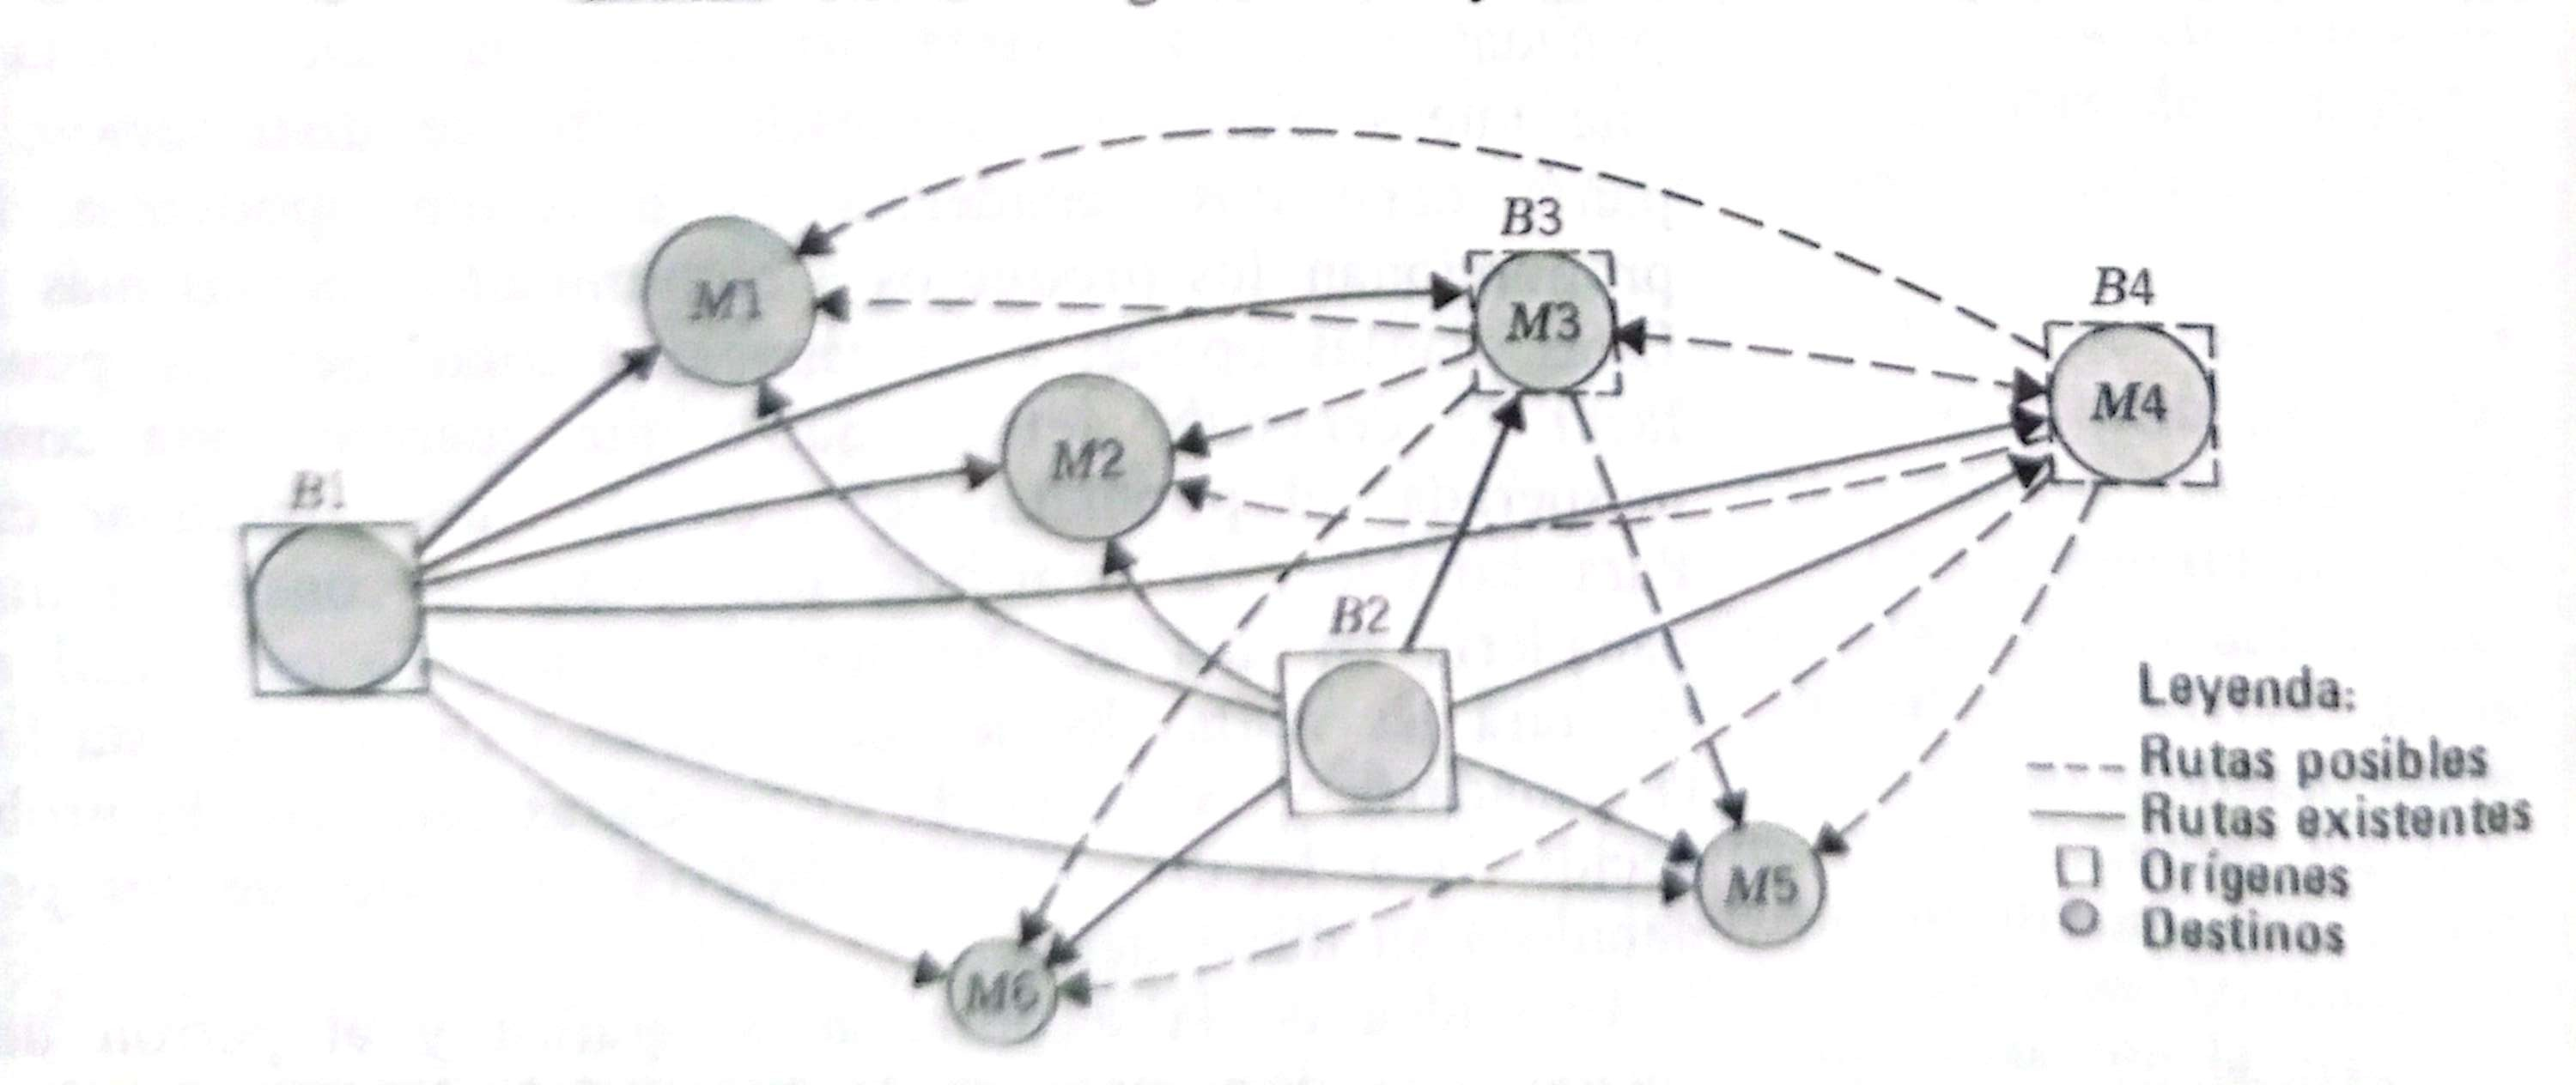
\includegraphics[width=0.8\textwidth]{image3.jpg}
\caption{Patrón existente de suministro y demanda en la red de distribución}
\label{fig:suministro_demanda}
\end{figure}

\begin{figure}[H]
\centering
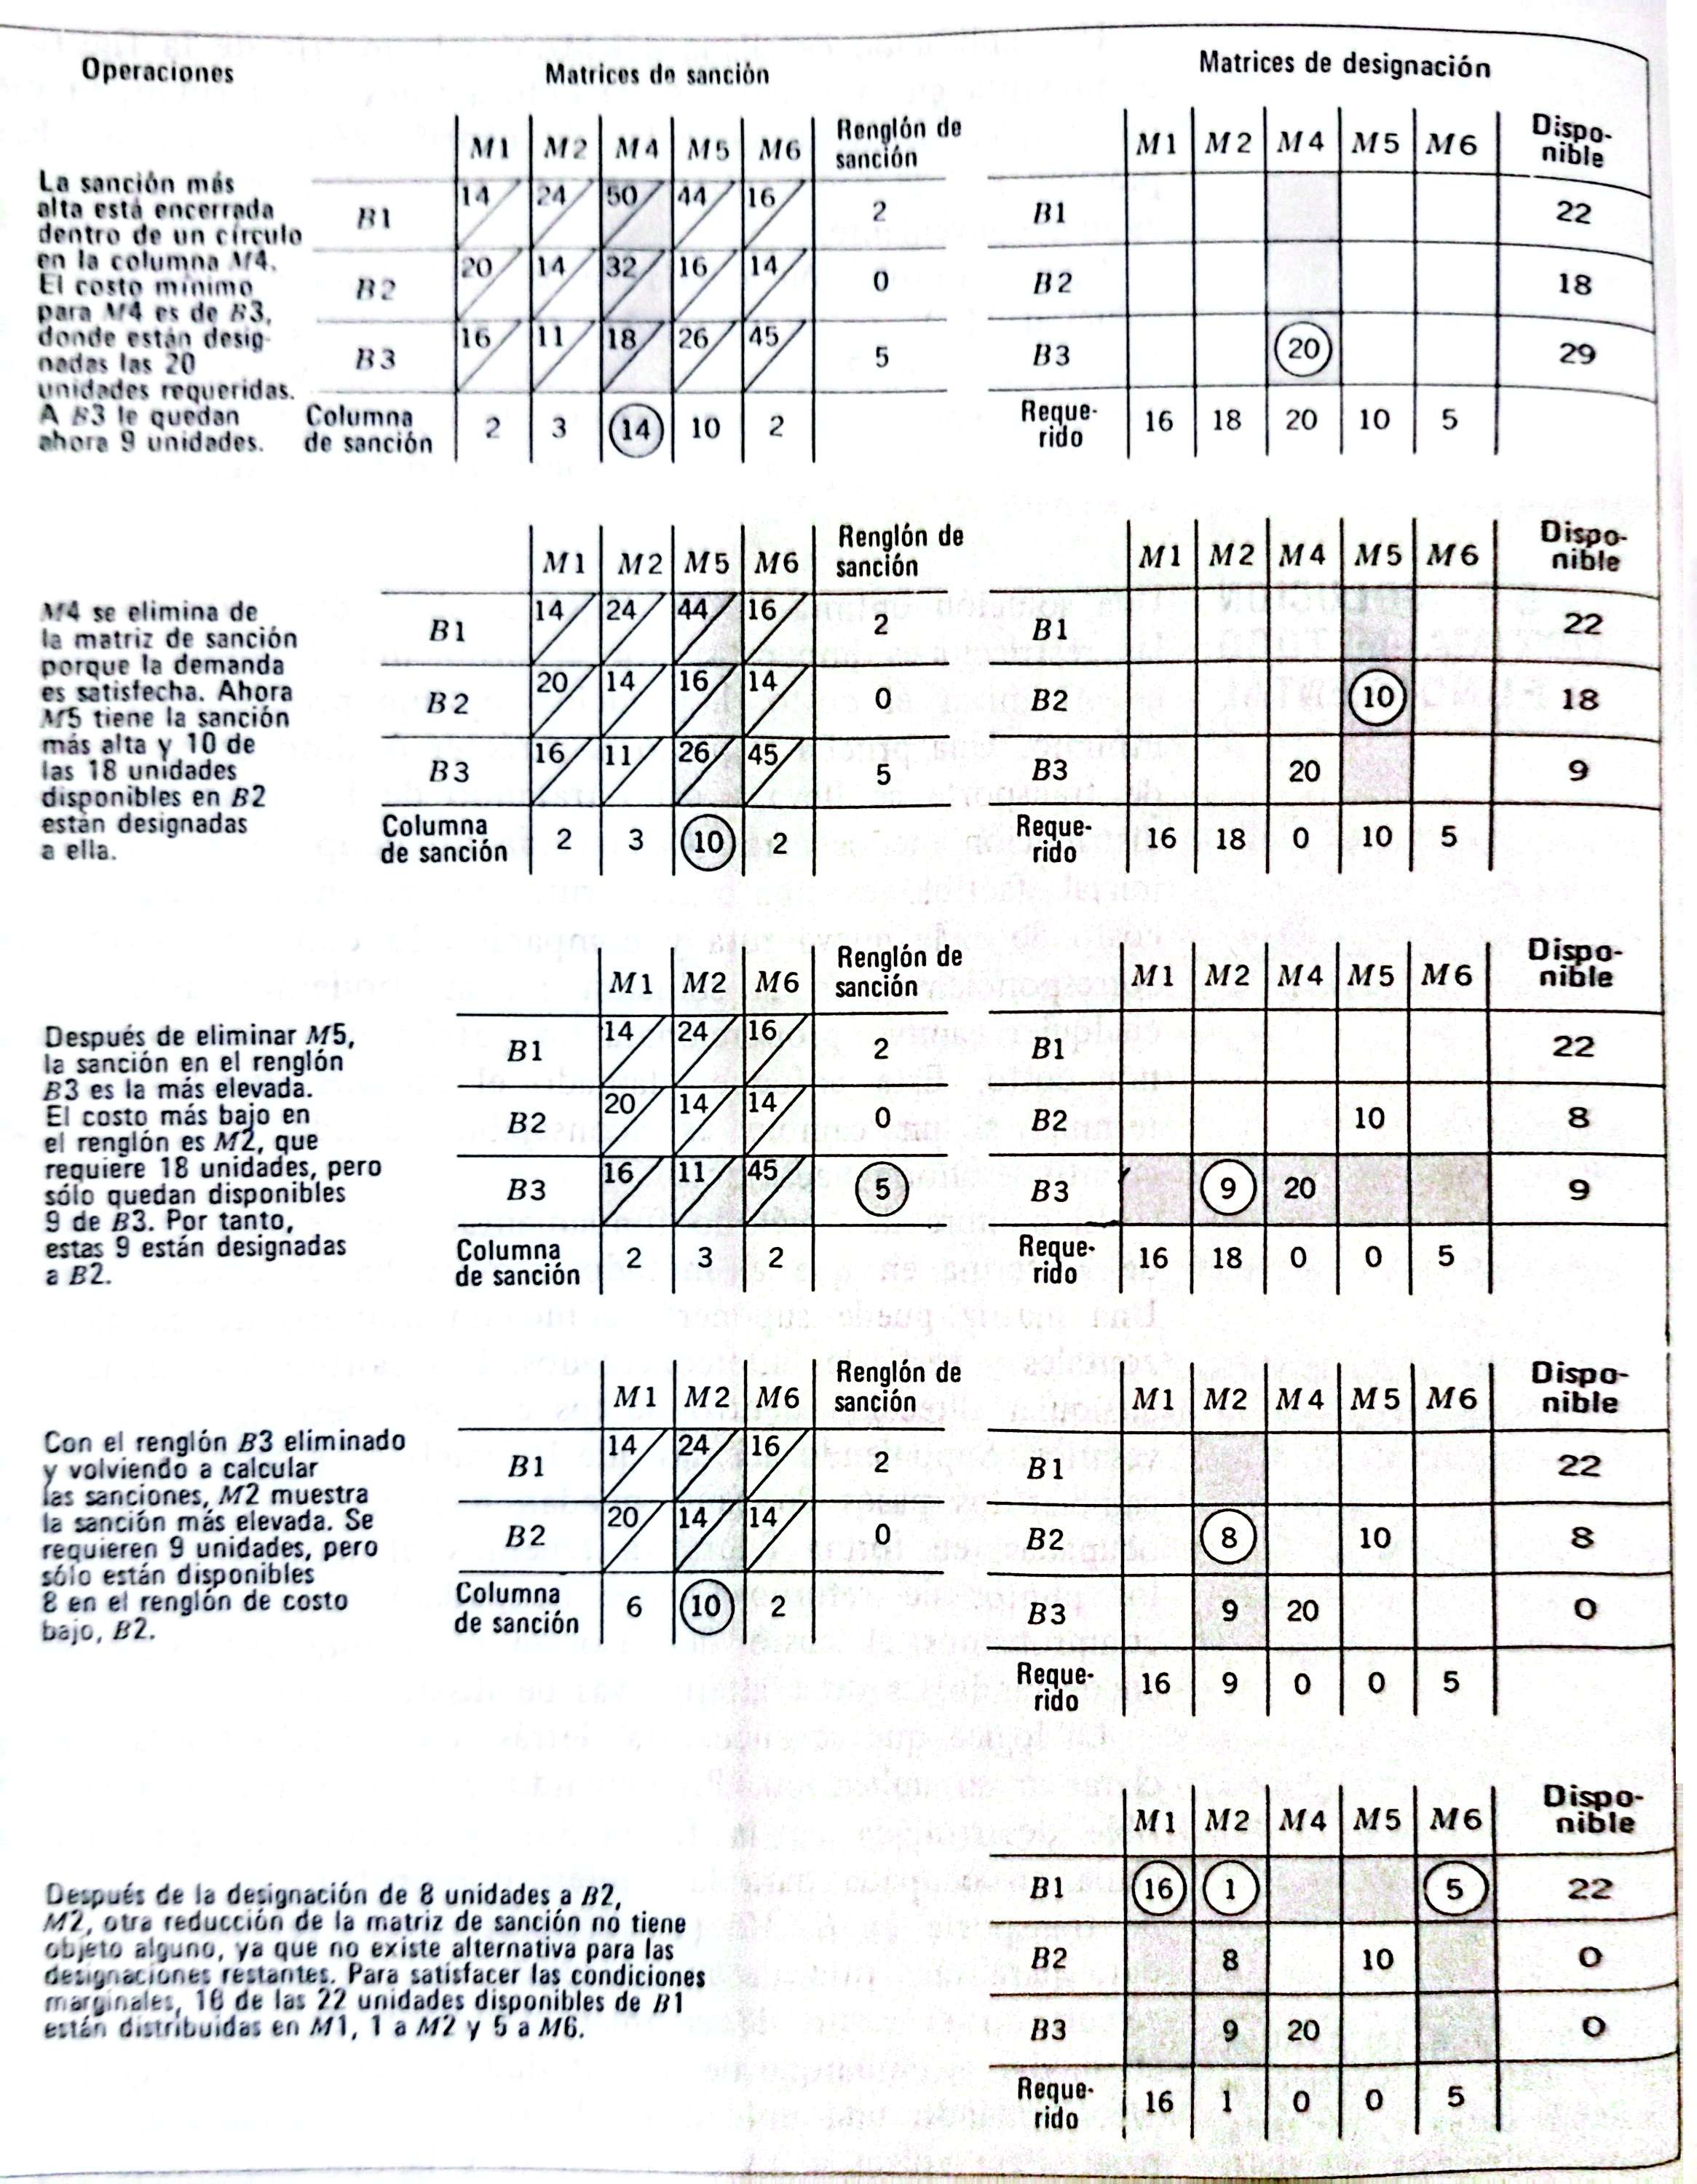
\includegraphics[width=0.8\textwidth]{image4.jpg}
\caption{Aplicación detallada del método de aproximación de Vogel a la red de distribución}
\label{fig:vogel_aplicacion}
\end{figure}

\begin{figure}[H]
\centering
\begin{minipage}{0.48\textwidth}
  \centering
  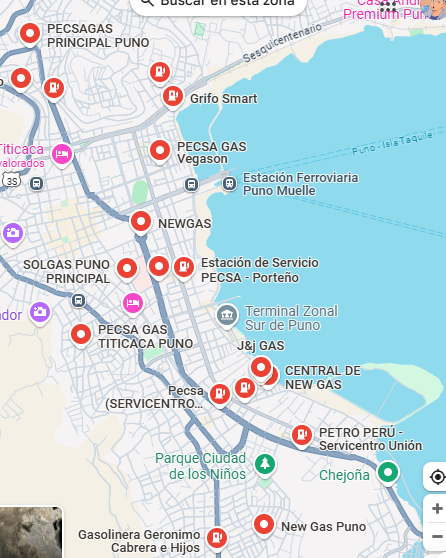
\includegraphics[width=0.9\textwidth]{gas.png}
  \caption{Ubicación de puntos de la empresa New Gas en Puno}
  \label{fig:gas_puntos}
\end{minipage}\hfill
\begin{minipage}{0.48\textwidth}
  \centering
  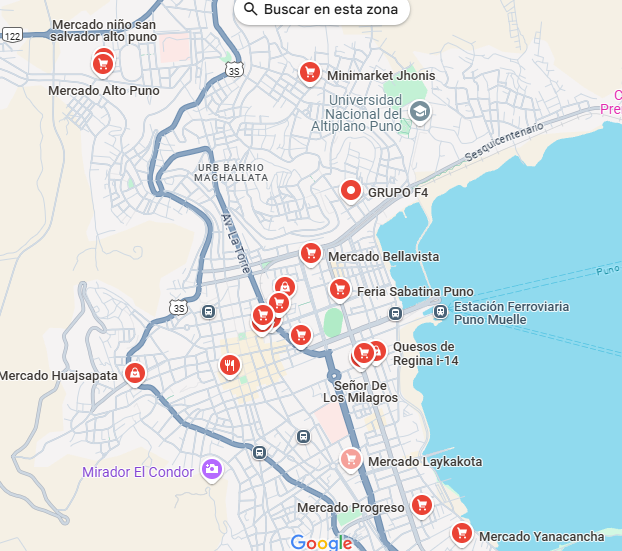
\includegraphics[width=0.9\textwidth]{mercado.png}
  \caption{Ubicación de los principales mercados en la región de Puno}
  \label{fig:mercados_puntos}
\end{minipage}
\end{figure}

\section{Datos del Problema}
En esta sección, presentamos los datos recopilados para el modelo de optimización de rutas de distribución de gas en la región de Puno. Estos datos provienen de un estudio de campo realizado en colaboración con distribuidoras locales de gas licuado de petróleo (GLP) \citep{OrozcoGutierrez2018}.

\subsection{Nodos de Distribución}
\begin{table}[H]
\centering
\begin{tabular}{|c|c|c|c|c|}
\hline
\textbf{Nodo} & \textbf{Tipo} & \textbf{Demanda} & \textbf{Capacidad Vehículo} & \textbf{Descripción} \\
\hline
0 & Origen (Planta) & N/A & 60 máx. & Planta central de distribución \\
\hline
1 & Mercado A & 10 & 50 & Mercado Central \\
\hline
2 & Mercado B & 10 & 50 & Mercado Bellavista \\
\hline
3 & Mercado C & 8 & 50 & Mercado Laykakota \\
\hline
4 & Mercado D & 15 & 50 & Mercado Internacional \\
\hline
\end{tabular}
\caption{Características de los nodos de distribución de gas}
\label{tab:nodos_distribucion}
\end{table}
\begin{figure}[H]
\centering
\begin{minipage}{0.48\textwidth}
  \centering
  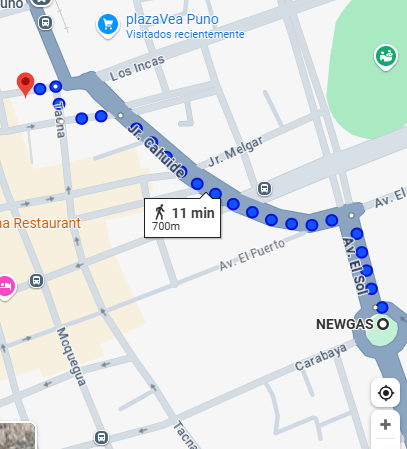
\includegraphics[width=0.9\textwidth]{central.png}
  \caption{Ubicación de la Empresa New Gas - Mercado Central}
  \label{fig:central}
\end{minipage}\hfill
\begin{minipage}{0.48\textwidth}
  \centering
  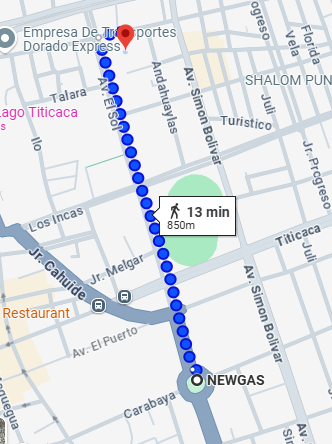
\includegraphics[width=0.9\textwidth]{bellavista.png}
  \caption{Ubicación de la Empresa New Gas - Mercado BellaVista}
  \label{fig:bellavista}
\end{minipage}
\end{figure}
\begin{figure}[H]
\centering
\begin{minipage}{0.48\textwidth}
  \centering
  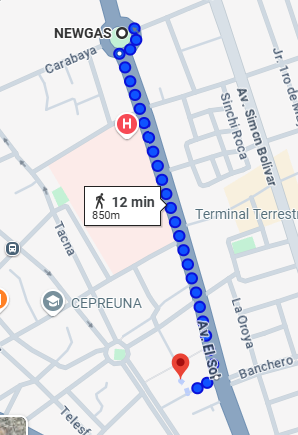
\includegraphics[width=0.9\textwidth]{laykakota.png}
  \caption{Ubicación de la Empresa New Gas - Mercado Laykakota}
  \label{fig:laykakota}
\end{minipage}\hfill
\begin{minipage}{0.48\textwidth}
  \centering
  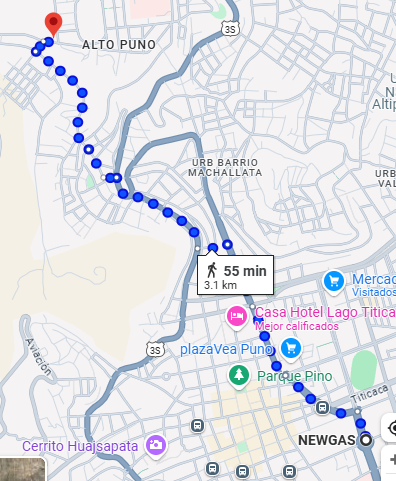
\includegraphics[width=0.9\textwidth]{altopuno.png}
  \caption{Ubicación de la Empresa New Gas - Mercado Central Alto Puno}
  \label{fig:altopuno}
\end{minipage}
\end{figure}

Según \citet{Cornejo2018}, la variabilidad en las demandas de los diferentes mercados refleja la diversidad económica y demográfica de la región de Puno. La capacidad de los vehículos se ha determinado considerando las restricciones de seguridad y eficiencia logística.

\subsection{Distancias entre Nodos}
\begin{table}[H]
\centering
\begin{tabular}{|c|c|c|c|c|c|}
\hline
\textbf{Desde} & \textbf{Hasta 0} & \textbf{Hasta A}& \textbf{Hasta B}& \textbf{Hasta C}& \textbf{Hasta D}\\
\hline
0 (Planta) & 0 & 0.7& 0.85& 0.85& 3.1\\
\hline
A& 0.7& 0 & 0.22& 1.4& 2.6\\
\hline
B& 0.85& 0.22& 0 & 1.7& 2.6\\
\hline
C& 0.85& 1.4& 1.7& 0 & 3.9\\
\hline
D& 3.1& 2.6& 2.5& 3.9& 0 \\
\hline
\end{tabular}
\caption{Distancias en kilómetros entre nodos de distribución}
\label{tab:distancias_nodos}
\end{table}

Las distancias han sido medidas utilizando sistemas de información geográfica (GIS) y corroboradas con datos de mapeo satelital \citep{Ballou2004}. Estas distancias son críticas para calcular los costos de transporte y optimizar las rutas.

\subsection{Costos de Transporte}
\begin{table}[H]
\centering
\begin{tabular}{|c|c|c|}
\hline

\textbf{Vehículo}& \textbf{Costo por km [S/]} & \textbf{Descripción} \\
\hline
Moto & 1.0 & Vehículo de carga ligera \\
\hline
Camioneta & 1.0& Vehículo de carga mediana \\
\hline
\end{tabular}
\caption{Costos de transporte por kilómetro para diferentes vehículos}
\label{tab:costos_transporte}
\end{table}

Los costos de transporte varían según el tipo de vehículo, considerando factores como consumo de combustible, mantenimiento y depreciación \citep{Chopra2018}.

\subsection{Capacidad de Vehículos}
\begin{table}[H]
\centering
\begin{tabular}{|c|c|}
\hline
\textbf{Vehículo} & \textbf{Capacidad (litros)} \\
\hline
Moto & 200 máx. \\
\hline
Camioneta & 3,000 máx. \\
\hline
\end{tabular}
\caption{Capacidad de carga de los vehículos de distribución}
\label{tab:capacidad_vehiculos}
\end{table}

La capacidad uniforme de los vehículos permite una planificación más estandarizada de las rutas, aunque en la práctica pueden existir variaciones menores \citep{Nahmias2014}.



\section{Parametrización del Modelo: 
 Aplicacion en la Distribucion de Gas }

A base de toda la informacion recolectada tenemos las siguientes rutas con sus costos y emisiones \citep{OrozcoGutierrez2018}:

\begin{table}[H]
\centering
\begin{tabular}{|c|c|c|}
\hline
\textbf{Ruta} & \textbf{Costo \( c_{ij} \)} & \textbf{Emisiones / kg \( s_{ij} \)}\\
\hline
1-2 & 56 & 0.72 \\
\hline
1-3 & 56 & 0.64 \\
\hline
2-3 & 56 & 0.68 \\
\hline
\end{tabular}
\caption{Parámetros de rutas }
\label{tab:rutas}
\end{table}

Los valores máximos en cada criterio son:
\begin{equation}
c_{\max} = 56, \quad s_{\max} = 0.72
\end{equation}

Normalizamos los datos siguiendo las recomendaciones de \citet{Winston2004}:

\begin{align}
c_{12}^\prime &= \frac{56}{56} = 1.00 \\
c_{13}^\prime &= \frac{56}{56} = 1.00 \\
c_{23}^\prime &= \frac{56}{56} = 1.00
\end{align}

\begin{align}
s_{12}^\prime &= \frac{0.72}{0.72} = 1.00 \\
s_{13}^\prime &= \frac{0.64}{0.72} \approx 0.89 \\
s_{23}^\prime &= \frac{0.68}{0.72} \approx 0.94
\end{align}

Se eligen las prioridades de acuerdo a \citet{Chopra2018}:

\begin{equation}
\alpha = 0.6, \quad \beta = 0.4
\end{equation}

Luego, la función objetivo ponderada es:

\begin{align}
Z &= \alpha \times (c_{12}^\prime x_{12} + c_{13}^\prime x_{13} + c_{23}^\prime x_{23}) \nonumber \\
&\quad + \beta \times (s_{12}^\prime x_{12} + s_{13}^\prime x_{13} + s_{23}^\prime x_{23}) \nonumber \\
&= 0.6 \times (1.00 x_{12} + 1.00 x_{13} + 1.00 x_{23}) \nonumber \\
&\quad + 0.4 \times (1.00 x_{12} + 0.89 x_{13} + 0.94 x_{23}) \nonumber \\
&= (0.6 \times 1.00 + 0.4 \times 1.00) x_{12} \nonumber \\
&\quad + (0.6 \times 1.00 + 0.4 \times 0.89) x_{13} \nonumber \\
&\quad + (0.6 \times 1.00 + 0.4 \times 0.94) x_{23} \nonumber \\
&= 1.00 x_{12} + 0.96 x_{13} + 0.98 x_{23}
\end{align}

\section{Formulación Matemática: Aplicacion en la Distribución de Gas}

\subsection{Variables de decisión}
\begin{itemize}[leftmargin=*]
    \item \( x_{ij} \in \{0,1\} \): 1 si se realiza la ruta de \(i\) a \(j\), 0 en caso contrario.
    \item \( q_j \geq 0 \): cantidad de gas transportada hacia el nodo \(j\).
\end{itemize}

\subsection{Datos del ejemplo}
\begin{align}
&\text{Costos:} \nonumber \\
& c_{12} = 56,\quad c_{13} = 56,\quad c_{23} = 56 \nonumber \\
& \text{Emisiones:} \nonumber \\
& s_{12} = 0.72,\quad s_{13} = 0.64,\quad s_{23} = 0.68 \nonumber
\end{align}

\subsection{Normalización}
\begin{equation}
c_{ij}^\prime = \frac{c_{ij}}{c_{\max}}, \quad s_{ij}^\prime = \frac{s_{ij}}{s_{\max}}
\end{equation}
\begin{align}
& c_{12}^\prime = 1.00,\quad c_{13}^\prime = 1.00,\quad c_{23}^\prime = 1.00 \nonumber \\
& s_{12}^\prime = 1.00,\quad s_{13}^\prime = 0.89,\quad s_{23}^\prime = 0.94 \nonumber
\end{align}

\subsection{Coeficientes de prioridad}
\begin{equation}
\alpha = 0.6,\quad \beta = 0.4
\end{equation}

\subsection{Función objetivo}
\begin{align}
\min Z &= \alpha \sum_{i,j} c_{ij}^\prime x_{ij} + \beta \sum_{i,j} s_{ij}^\prime x_{ij} \nonumber \\
&= 0.6 (1.00 x_{12} + 1.00 x_{13} + 1.00 x_{23}) + 0.4 (1.00 x_{12} + 0.89 x_{13} + 0.94 x_{23}) \nonumber \\
&= 1.00 x_{12} + 0.96 x_{13} + 0.98 x_{23}
\end{align}

\subsection{Restricciones}
\begin{align}
& \text{Satisfacción de demanda en nodos 2 y 3:} \nonumber \\
& q_2 \geq 50 \nonumber \\
& q_3 \geq 30 \nonumber
\end{align}

\begin{align}
& \text{Capacidad del vehículo:} \nonumber \\
& q_2 + q_3 \leq 80 y \nonumber \\
& y \in \{0,1\} \nonumber
\end{align}

\begin{align}
& \text{Balance de flujo en los nodos:} \nonumber \\
& x_{12} \cdot q_1 - x_{23} \cdot q_2 = 50 \nonumber \\
& x_{13} \cdot q_1 + x_{23} \cdot q_2 = 30 \nonumber
\end{align}

\begin{align}
& \text{Variables binarias:} \nonumber \\
& x_{ij} \in \{0,1\} \nonumber
\end{align}

\begin{figure}[H]
\centering
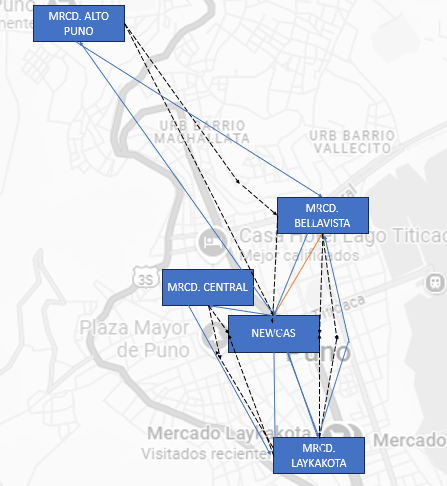
\includegraphics[width=0.8\textwidth]{Captura de pantalla 2025-05-14 122727.png}
\caption{caminos optimizados con respecto a la oferta y demanda}
\label{fig:optimizacion}
\end{figure}

\section{Conclusiones}
La implementación de un modelo de programación lineal mixta para la optimización de rutas de distribución de gas en la región de Puno ofrece una solución eficiente a un problema logístico complejo. Este enfoque permite:

\begin{itemize}[leftmargin=*]
    \item Minimizar los costos operativos mientras se consideran factores ambientales y de seguridad
    \item Satisfacer las demandas de todos los puntos de consumo de manera oportuna
    \item Utilizar eficientemente los recursos disponibles, especialmente los vehículos de transporte
\end{itemize}

Los resultados de este trabajo pueden servir como base para futuras investigaciones en el campo de la logística de distribución de combustibles en regiones con características geográficas y socioeconómicas similares a las de Puno \citep{Cornejo2018}.

\section{Recomendaciones}
Basados en el desarrollo de este trabajo, se recomienda:

\begin{enumerate}[label=\arabic*., leftmargin=*]
    \item Implementar el modelo propuesto en un software especializado de optimización como GAMS, AMPL o Python con la biblioteca PuLP
    \item Extender el modelo para incluir variaciones estacionales en la demanda y condiciones climáticas
    \item Integrar sistemas de información geográfica (GIS) para una representación más precisa de las rutas y condiciones de tránsito
\end{enumerate}

\bibliographystyle{apalike}
\bibliography{referencias}

% Contenido del archivo referencias.bib
\begin{filecontents}{referencias.bib}
@book{Hillier2010,
  author = {Hillier, Frederick S. and Lieberman, Gerald J.},
  title = {Introducción a la Investigación de Operaciones},
  year = {2010},
  publisher = {McGraw-Hill},
  address = {México},
  edition = {9na}
}

@book{Taha2017,
  author = {Taha, Hamdy A.},
  title = {Investigación de Operaciones},
  year = {2017},
  publisher = {Pearson},
  address = {México},
  edition = {10ma}
}

@book{Ballou2004,
  author = {Ballou, Ronald H.},
  title = {Logística: Administración de la cadena de suministro},
  year = {2004},
  publisher = {Pearson Educación},
  address = {México},
  edition = {5ta}
}

@book{Nahmias2014,
  author = {Nahmias, Steven},
  title = {Sistemas de Producción: Planeación, Análisis y Control},
  year = {2014},
  publisher = {McGraw-Hill},
  address = {México},
  edition = {6ta}
}

@book{Winston2004,
  author = {Winston, Wayne L.},
  title = {Investigación de Operaciones: Aplicaciones y Algoritmos},
  year = {2004},
  publisher = {Thomson},
  address = {México},
  edition = {4ta}
}

@book{Chopra2018,
  author = {Chopra, Sunil and Meindl, Peter},
  title = {Administración de la cadena de suministro: Estrategia, planeación y operación},
  year = {2018},
  publisher = {Pearson},
  address = {México},
  edition = {6ta}
}

@book{Dekker2012,
  author = {Dekker, Rommert and Bloemhof, Jacqueline and Mallidis, Ioannis},
  title = {Operations Research for green logistics – An overview of aspects, issues, contributions and challenges},
  journal = {European Journal of Operational Research},
  year = {2012},
  volume = {219},
  number = {3},
  pages = {671-679}
}

@article{OrozcoGutierrez2018,
  author = {Orozco Gutiérrez, Alberto and Martínez Ramírez, Javier},
  title = {Aplicación de la programación lineal para la optimización del sistema de distribución de GLP en la sierra peruana},
  journal = {Revista Peruana de Ingeniería},
  year = {2018},
  volume = {10},
  number = {2},
  pages = {45-62}
}

@article{Cornejo2018,
  author = {Cornejo, Luis and Rodriguez, María and Palacios, Ricardo},
  title = {Desafíos logísticos en la distribución de combustibles en zonas altoandinas del Perú},
  journal = {Revista Andina de Estudios de la Cadena de Suministro},
  year = {2018},
  volume = {3},
  number = {1},
  pages = {78-95}
}


\end{filecontents}

\section{ANEXOS}
\subsection{ANEXO: EVIDENCIAS}
% aqui se insertan imagenes:
% evidencia1.png
% evidencia2.png
\begin{figure}[H]
\centering
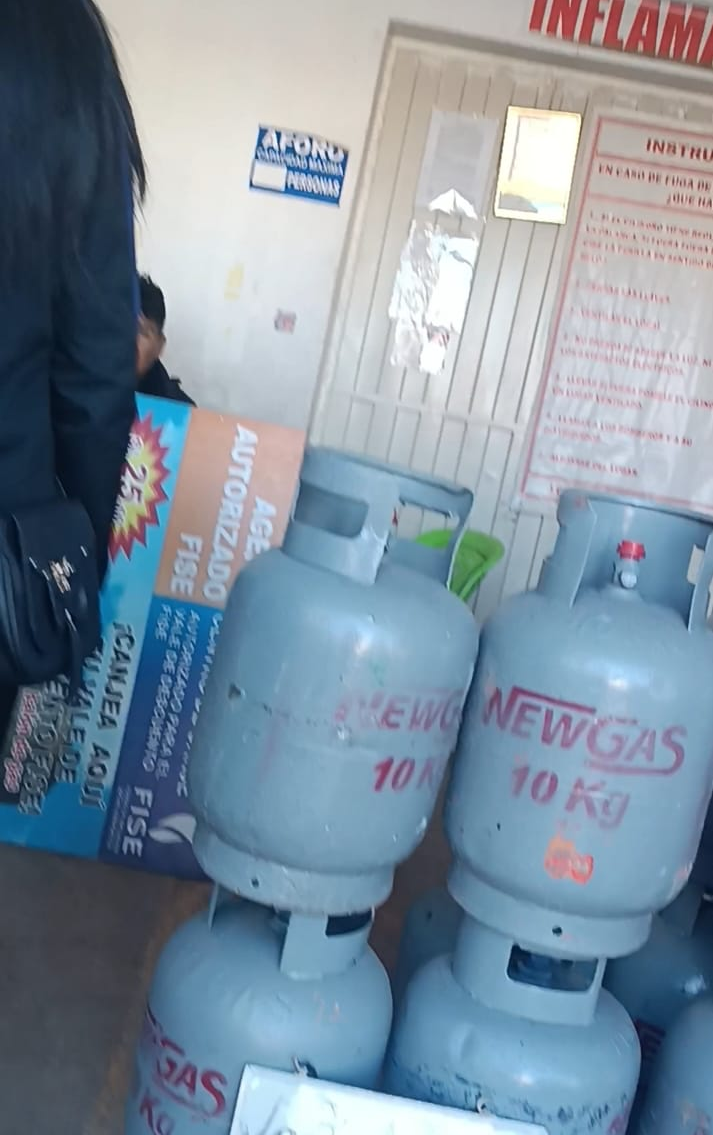
\includegraphics[width=0.8\textwidth]{evidencia.png}
\end{figure}

\begin{figure}[H]
\centering

\includegraphics[width=0.8\textwidth]{evidencia2.png}
\end{figure}
\end{document}